%--------------------------------------------------------------------------------
%\documentclass{article}

\documentclass[a4paper, 16pt]{article}
\usepackage[T1]{fontenc}
\usepackage{hyperref}
\usepackage[all]{hypcap}
\usepackage[utf8]{inputenc}
\usepackage{graphicx}
\usepackage[left=2cm, top=3cm, text={17cm, 24cm}]{geometry}
\usepackage[czech, english]{babel}
\selectlanguage{english}
\usepackage{subfig}                % \subfloat
\usepackage{color}
\usepackage{url}
\inputencoding{utf8}
\usepackage{float}
%\usepackage[bf]{caption2}
\usepackage{hyperref}
\usepackage[all]{hypcap}
\hypersetup{colorlinks=false, linkbordercolor=1 1 1, citebordercolor=1 1 1}
\usepackage[right]{lineno}
\renewcommand\linenumberfont{\normalfont\tiny\color{blue}}


\title{Paraphrase - detekce vztahů vět v textu}
\author{Matej Berezný <xberez03@stud.fit.vutbr.cz>\\
Ondrej Valo <xvaloo00@stud.fit.vutbr.cz>\\
Miloš Uriga <xuriga00@stud.fit.vutbr.cz>}
\date{\today}


%--------------------------------------------------------------------------------


\begin{document}
\selectlanguage{czech}
\maketitle

\section{Úvod}
\label{uvod}
Cieľom projektu bolo vytvoriť program pre klasifikáciu duplikátov otázok. Ako nástroj pre daný účel sme sa rozhodli využiť transformer model BERT. Dodatočne bolo toto zadanie rozšírené o pridanie modifikácií pre danú architektúru a porovnanie s existujúcimi riešeniami.


%%%%%%%%%%%%%%%%%%%%%%%%%%%%%%%%%%%%%%%%%%%%%%%%%%%%%%%%%%%%%%%%%%%%%%%%%%%%%%%%%%%%%%%%

\section{Dataset}
\label{dataset}
Ako dataset bol využitý Quora Question Pairs dataset \cite{quora}. Jedná sa o klasifikačný problém o dvoch triedach kde buď dve otázky boli duplikáty alebo nie. Dáta obsahovali 6 stĺpcov uvedených v tabuľke \ref{table:data} aj s príkladom obsahu.
\begin{table}[H]
\centering
\begin{tabular}{ |c|c|c|c|c|c| } \hline
id & qid1 & qid2 & question1 & question2 & is\_duplicate\\ \hline
38 & 75 & 76 & How do we prepare for UPSC? & How do I prepare for civil service? & 1\\ \hline
\end{tabular}
\caption{Hlavička dátovej sady}
\label{table:data}
\end{table}
\begin{itemize}
    \item id - identifikačné číslo data
    
    \item qid1 - identifikačné číslo prvej otázky
    
    \item qid2 - identifikačné číslo druhej otázky
    
    \item question1 - prvá otázka na porovnanie
    
    \item question2 - druhá otázka na porovnanie
    
    \item is\_duplicate - 1 pre duplikátne otázky 0 pre nie
\end{itemize}


\section{Augmentácia}
\label{augmentation}
Augmentácia predstavená v štúdií \cite{augmentation} popísaná v podsekciách \ref{SR}, \ref{RI}, \ref{RS} a v \ref{RD}. Tento spôsob augmentácie sme zvolili preto, že autorom vyššie spomínanej štúdie priniesla výrazné zlepšenie v presnosti trénovaných sietí. Rozhodli sme sa preto teda otestovať, či aplikovanie takejto augmentácie zlepší aj výsledky hľadania duplicitných otázok, poprípade či bude mať aplikácia takejto augmentácie na 'cutting-edge' modely typu BERT pozitívny vplyv na ich efektivitu. Rovnako ako v \cite{augmentation} bola augmentácia prevádzaná na vetách podla dĺžky viet kde počet augmentácií $n$ bol počítaný nasledovne: $n = l \times p$ kde $l$ predstavuje dĺžku vety a $p$ predstavuje pravdepodobnosť aplikovania augmentácia. Taktiež sme v augmentácií využili parameter $N$ ktorí určoval celkový počet augmentovaných viet na jednu pôvodnú vetu.

\subsection{Zámena synoným (SR)}
\label{SR}
Augmentačná technika kde boli zamieňané náhodné slová vo vete za ich synonymá. Avšak tieto slová nemohli byť takzvané "stopwords". Čo je určitá skupina slov ktoré filtrujeme pre nezvyšovanie zbytočného šumu v rámci dát, medzi takéto v našom prípade patria napríklad 'i', 'me', 'my', 'myself', 'we', 'our' \cite{stop_words}. Pre hľadanie synoným bol použitý natrénovaný model wordnet \cite{wordnet}. Kde následne na základe vstupnej pravdepodobnosti sa augmentovali vety 1 krát alebo viac a pridali k ostatným augmentovaným vetám. Príklad takejto augmentácie možno vidno v \ref{table:SR}. 

\begin{table}[H]
\centering
\begin{tabular}{ |c|c| } \hline
pôvodná veta: & A sad, superior human comedy played out on the back roads of life\\ \hline
augmentovaná veta: & A \textbf{lamentable}, superior human comedy played out on the \textbf{backward} road of life. \\ \hline
\end{tabular}
\caption{Príklad zámeny synonymom}
\label{table:SR}
\end{table}

\subsection{Náhodné vsunutie (RI)}
\label{RI}
Táto technika funguje podobným spôsobom ako \ref{SR}, kde narozdiel nahradzovania slov za synonymá, sa tieto synonymá vkladajú do pôvodnej vety. Príklad takejto augmentácie možné pozorovať v tabuľke \ref{table:RI}.

\begin{table}[H]
\centering
\begin{tabular}{ |c|c| } \hline
pôvodná veta: & A sad, superior human comedy played out on the back roads of life\\ \hline
augmentovaná veta: & A sad, superior human comedy played out on \textbf{funniness} the back roads of life.\\ \hline
\end{tabular}
\caption{Príklad vkladania synonyma do vety}
\label{table:RI}
\end{table}

\subsection{Náhodná zámena (RS)}
\label{RS}
Tu augmentácia prebiehala spôsobom že z dát sa vyberú dve slová z danej vety a vymenia si svoje pozície. Táto technika sa taktiež vykoná 1 krát a viac podľa dĺžky vety a určenej pravdepodobnosti. Príklad takejto augmentácie je možné pozorovať v tabuľke \ref{table:RS}.

\begin{table}[H]
\centering
\begin{tabular}{ |c|c| } \hline
pôvodná veta: & A sad, superior human comedy played out on the back roads of life\\ \hline
augmentovaná veta: & A sad, superior human comedy played out on \textbf{roads} back \textbf{the} of life\\ \hline
\end{tabular}
\caption{Príklad zámeny slov vo vete}
\label{table:RS}
\end{table}

\subsection{Náhodné zmazanie (RD)}
\label{RD}
V tejto augmentačnej technike sa prechádzajú všetky slová a každé má pravdepodobnosť byť z vety odstránené. Pravdepodobnosť je ručne nastavovaná a rovnaká pre každé slovo v danej vete. Príklad takejto augmentácie je možné pozorovať v tabuľke \ref{table:RD}.

\begin{table}[H]
\centering
\begin{tabular}{ |c|c| } \hline
pôvodná veta: & A sad, superior human comedy played out on the back roads of life\\ \hline
augmentovaná veta: & A sad, superior human out on the roads of life\\ \hline
\end{tabular}
\caption{Príklad odstránenia slov vo vete}
\label{table:RD}
\end{table}

\section{Architektúra}
\label{architektura}

Architektúry využité v tomto projekte sú opísané v nasledujúcivh podsekciách BERT v \ref{BERT_a}, LSTM v \ref{LSTM_a}, CNN v \ref{CNN_a} a LSTMCNN v \ref{LSTMCNN_a}. Dôvodom využitia všetkých modelov v siamese sieťach je z dôvodu povahy problému, kde naše dáta sa skladajú z 2 otázkou a 1 labelu. Kde vstupné sekvencie na uvedených modeloch \ref{fig:3}, \ref{fig:4}, \ref{fig:5}, \ref{fig:6} boli páry otázok kde každá sekvencia bola jedna z otázka.

\subsection{BERT}
\label{BERT_a}
Na implementáciu BERTu bola využitá knižnica transformers \cite{transformers}, kde pre siamese verziu sme museli preťažovať niektoré funkcie pre trénovanie. V obrázku \ref{fig:3}, input sequence predstavujú otázky pre porovnávanie. Tokenizer je taktiež využitý z knižnice transformers ktorý danú vetu zakóduje, jeho vstup a výstup je možno vidieť v tabulke \ref{table:tokenizer}.

\begin{table}[H]
\centering
\begin{tabular}{ |c|c| } \hline
Vstupná veta: & where is Himalayas in the world map?\\ \hline
Zakódovaná veta : & [101, 2073, 2003, 26779, 1999, 1996, 2088, 4949, 1029, 102]\\ \hline
kódovanie na tokeny : & ['[CLS]', 'where', 'is', 'himalayas', 'in', 'the', 'world', 'map', '?', '[SEP]']\\ \hline
\end{tabular}
\caption{Príklad fungovania tokenizeru}
\label{table:tokenizer}
\end{table}

Model BERT je navrhnutý tak, že veta musí začínať tokenom [CLS] a končiť tokenom [SEP]. Kde keď pracujeme s viacerými vetami na vstupe tak je potreba oddeľovať vety tokenom [SEP], ale vďaka knižnici Hugging-face to knižnica tokenizerov robí za nás.
Vďaka tejto vlastnosti sme okrem Siamese BERT trénovali aj samotný BERT ktorých výsledky možno vidieť v sekcii \ref{vyhodnotenie}

\begin{figure}[H]
    \centering
    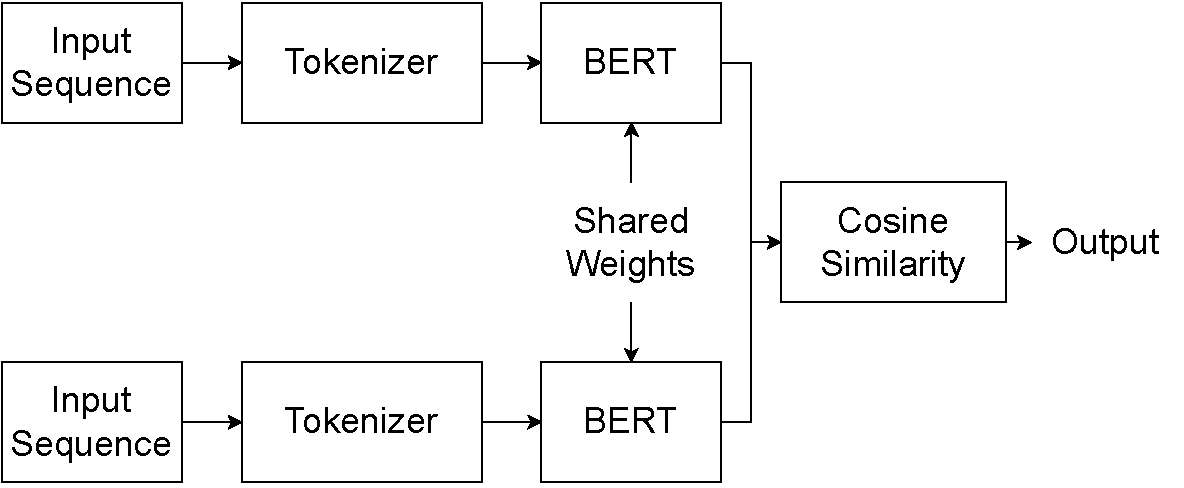
\includegraphics[width=15cm]{imgs/BERT.pdf}
    \caption{Schéma modelu Siamese BERT}
    \label{fig:3}
\end{figure}

\subsection{LSTM}
\label{LSTM_a}
Rovnako ako v predchádzajúcej sekcií každá vstupná sekvencia predstavuje jednú otázku. Tie sú posielané na vstup Glove embeddingu ktorý nám dá vektory reprezentujúce slová vo vete, tie sa ďalej posielajú cez dve obojsmerné skryté vrstvy LSTM sieti a výsledky sa porovnávajú pomocou Cosine similarity. Každá s LSTM vrstviev ma hodnotu \texttt{hidden\_size} nastavenú na 50.
\begin{figure}[H]
    \centering
    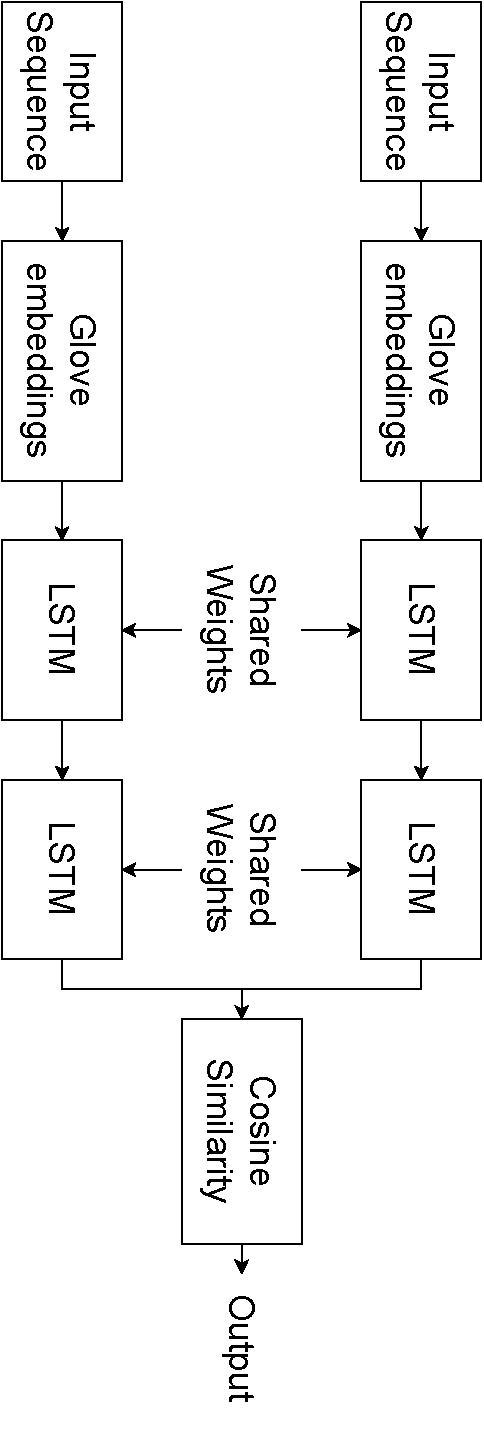
\includegraphics[width=5cm, angle =90 ]{imgs/LSTM.pdf}
    \caption{Schéma modelu Siamese LSTM}
    \label{fig:4}
\end{figure}

\subsection{CNN}
\label{CNN_a}
Rovnako ako v \ref{LSTM_a}, boli vstupné sekvencie posieláne do Glove embeddings pre reprezentáciu slov vektormi. Glove embeddings boli v každom modeli trénované zároveň s modelom. Následne boli vektory posielané konvolučných neurónových sietí, skladajúcich sa z 4 vrstiev konvolúcie nasledovaných aktivačnými vrstvami, kde za každou vrstvou konvolúcie nasleduje aktivačná funkcia, pričom veľkosti filtrov jednotlivých konvolučných vrstiev sú, dvakrát  $5 \times 100$ a dvakrát $3 \times 100$. Pre zníženie tzv. 'overfittingu' sme nakoniec pridali jednu \texttt{dropout} vrstvu s šancou \texttt{0.3}.
\begin{figure}[H]
    \centering
    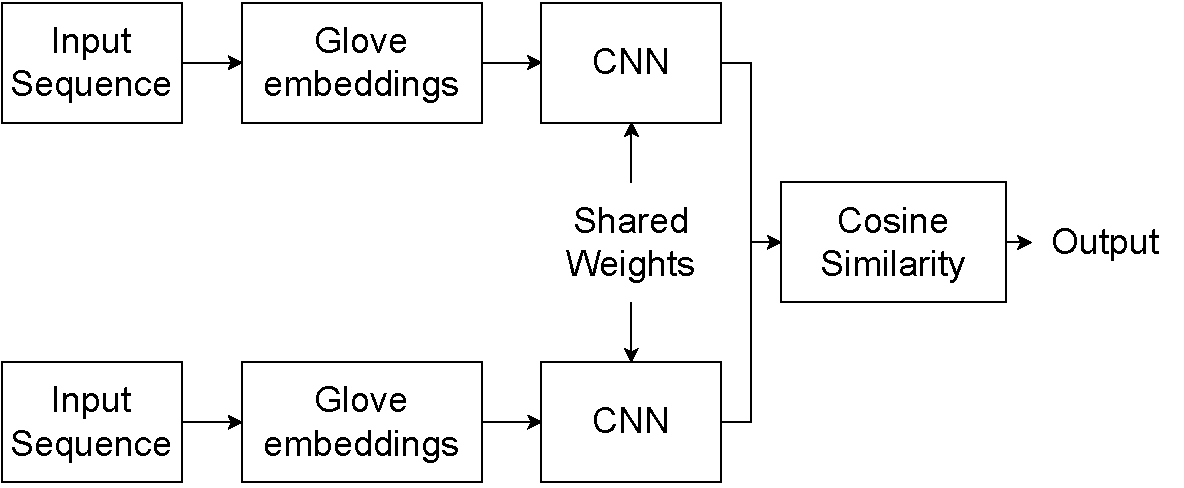
\includegraphics[width=15cm]{imgs/CNN.pdf}
    \caption{Schéma modelu Siamese CNN}
    \label{fig:5}
\end{figure}

\subsection{LSTM CNN}
\label{LSTMCNN_a}
Ako môžeme pozorovať na obrázku \ref{fig:6}, LSTMCNN skladá sa z dvoch CNN so zdielanými váhami a dvoch LSTM taktiež s zdielanými váhami, kde vstupy sú rovnaké ako v predchádzajúcich modeloch, a výstupy týchto LSTM a CNN sú spájané a posielané do vrstvy pre porovnanie podobnosti. V tomto modele sa konvolučné siete skladajú z jednej vrstvy konvolúcie, aktivačnej ReLU funkcie nasledovanej 'dropout' vrstvou pre zníženie šance na 'overfitting', pričom parametre konvolučného filtra sú $5 \times 100$ a šanca pre 'dropout' je nastavená na \texttt{0.3}.

\begin{figure}[H]
    \centering
    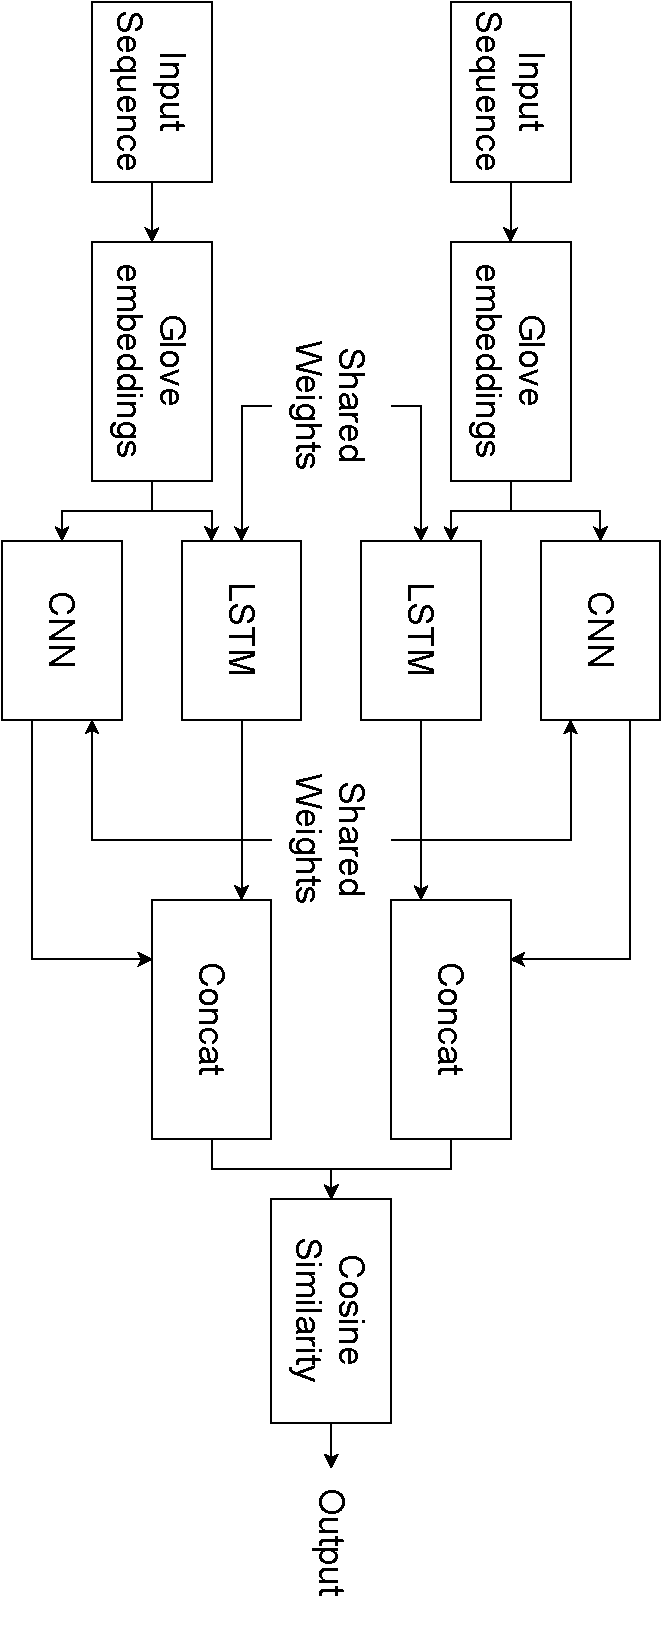
\includegraphics[width=5cm, angle =90 ]{imgs/LSTM_CNN.pdf}
    \caption{Schéma modelu Siamese LSTMCNN}
    \label{fig:6}
\end{figure}

%%%%%%%%%%%%%%%%%%%%%%%%%%%%%%%%%%%%%%%%%%%%%%%%%%%%%%%%%%%%%%%%%%%%%%%%%%%%%%%%%%%%%%%%

\section{Vyhodnotenie}
\label{vyhodnotenie}

Boli vykonané dve sady testov, prvá sada bola zameraná na skúmanie vplyvu augmentácie na celkovú presnosť siete pri použití iba čiastkovej trénovacej sady a druhá sada skúmala celkovú presnosť sietí po natrénovaní na celkom datasete. 

\subsection{Vyhodnotenie augmentácie}
\subsubsection{BERT}
Oba modely typu BERT (\texttt{Siamese} a \texttt{Classifier}) boli dotrénované po dobu 4 epoch na štyroch rôznych velkostiach trénovacej sady \texttt{size\_of\_train = [500, 2000, 5000]} rovnako ako v študíí o augmentácií. Takisto boli pre každú trénovaciu sadu vyskúšané 4 rôzne intenzity augmentácie \texttt{aug\_intensity}, a to \texttt{0} - žiadna augmentácia, slúžiaca ako základ pre porovnávanie a následne \texttt{3}, \texttt{6}, \texttt{9} (číslo reprezentuje počet nových otázkových párov vzniknutých po augmentácií). Ako strátová funkcia bola použitá \texttt{MeanSquareError}, ako optimiser \texttt{Adam} a na overenie celkovej presnosti sme použili metriku \texttt{accuracy\_score} z knižnice \texttt{sklearn}.

\begin{figure}[H]
    \centering
    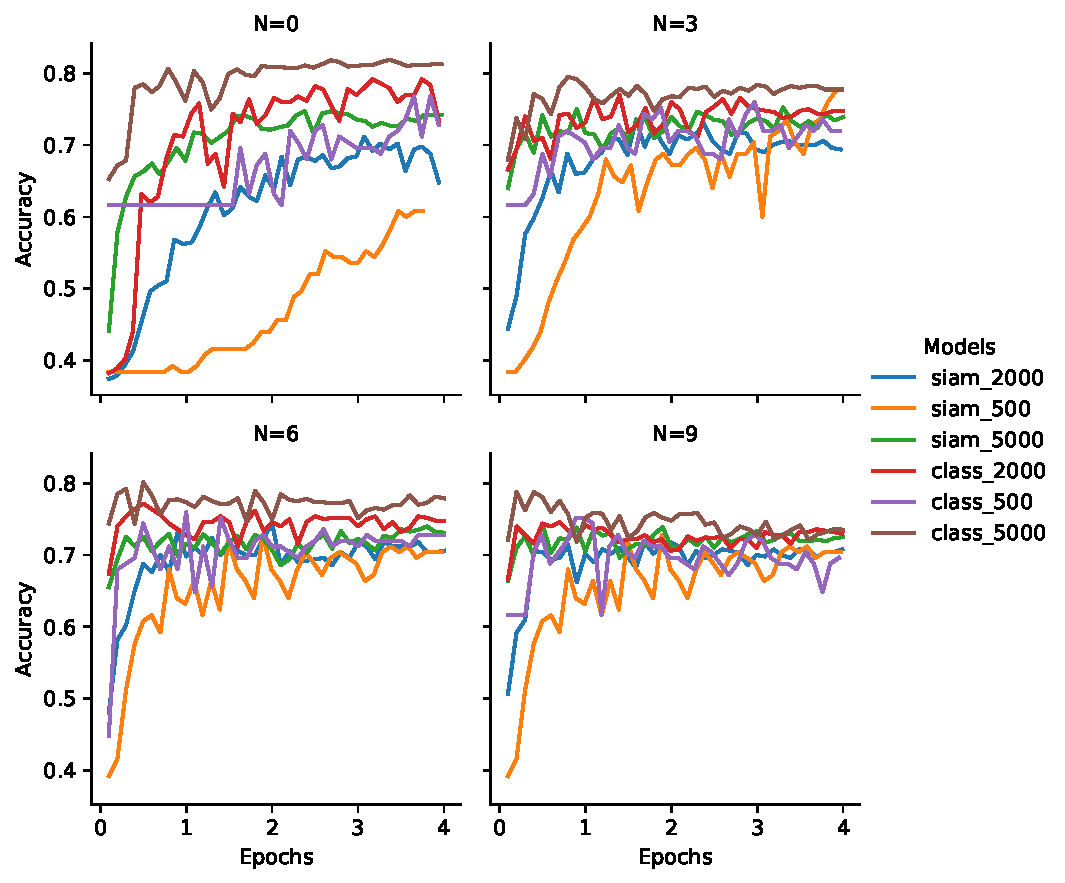
\includegraphics[width=15cm]{imgs/BERT_graph.pdf}
    \caption{Hodnota \texttt{accuracy\_score} vypočítaná na evaluačnej sade počas trénovania modelov BERT v jednotlivých epochách}
    \label{fig:1}
\end{figure}

Z grafov znázornených na obrázku \ref{fig:1} je možné si všimnúť, že akákoľvek augmentácia mala pri väčšom množstve trénovacích vzoriek v najlepšom prípade neutrálny efekt a v tom horšom viedla k zníženiu celkovej presnosti siete typu BERT. Pri malom množstve dát je možné si povšimnúť rýchlejšiu konvergenciu a miestami vyššiu presnosť sietí trénovaných na augmentovaných dátach, pričom najlepšie výsledky dosahovali siete, pri ktorých bola intensita augmentácie \texttt{aug\_intensity} nastavená na hodnotu \texttt{3}.  

\subsubsection{Ostatné modely}
Pred tým, než bude možné prehlásiť, že spôsob augmentácie implementovaný v tomto projekte nemá pozitívny vplyv na presnosť predikcie podobnosti otázok, bolo nutné ho ešte vyskušať na modeloch, ktoré neboli predom natrénované na vysokom množstve dát. Preto sme rovnaké testy vykonali aj na menších modeloch \texttt{LSTM}, \texttt{CNN} a \texttt{LSTMCNN}, ktoré boli natrénované po dobu 25 epoch. Zvyšné parametre trénovania sú identické s trénovaním modelov typu BERT. 

\begin{figure}[H]
    \centering
    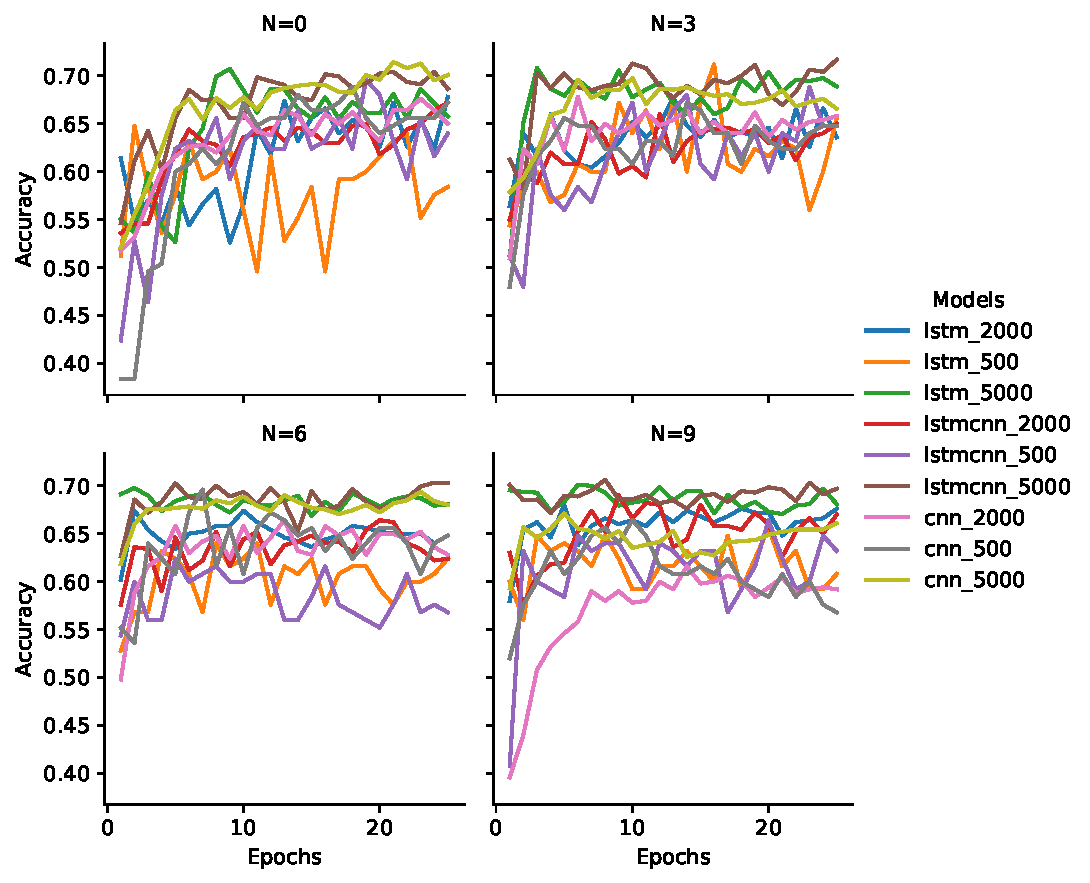
\includegraphics[width=15cm]{imgs/NN_graph.pdf}
    \caption{Hodnota \texttt{accuracy\_score} vypočítaná na evaluačnej sade počas trénovania siamských modelov v jednotlivých epochách}
    \label{fig:2}
\end{figure}

Z výsledkov grafov na obrázku \ref{fig:2} vyplýva, že narozdiel od modelov BERT použitie augmentácie pri menších modeloch prinieslo zrýchlenie konvergencie a malé zlepšenie presnosti na evaluačnej sade aj s väčšim množstvom trénovacích dát. Zároveň sa potvrdilo predošlé pozorovanie, že nižšia úroveň intenzity augmentácie (\texttt{aug\_intensity} = \texttt{3}) dosahuje lepších výsledkov, keďže pri vyšších hodnotách už nastáva 'overfitting' na trénovacích dátach.

\subsubsection{Celkové výsledky}

V konečnom dôsledku však na základe dát z tabuľky \ref{table:ResultsAUG} môžeme vyvodiť, že augmentácia mala neutrálny až miestami negatívny vplyv na celkovú presnosť siete na testovacích dátach - či už pri dotrénovaných modeloch typu BERT, alebo nami implementovaných modeloch \texttt{LSTM}, \texttt{LSTMCNN}, \texttt{CNN}.

\begin{table}[H]
\centering
\begin{tabular}{ |c|c|c|c|c|c|c| } \hline
Samples & Aug. intensity & siam\_bert & class\_bert & siam\_cnn & siam\_lstm & siam\_lstmcnn\\ \hline
500 & 0 & 0.59 & 0.73 & 0.59 & 0.43 & 0.64\\
  & 3 & 0.66 & 0.72 & 0.64 & 0.59 & 0.64 \\
  & 6 & 0.67 & 0.71 & 0.61 & 0.62 & 0.64 \\
  & 9 & 0.68 & 0.70 & 0.60 & 0.64 & 0.63 \\ \hline
2000  & 0 & 0.69 & 0.77 & 0.69 & 0.67 & 0.67 \\
  & 3 & 0.69 & 0.75 & 0.66 & 0.64 & 0.68 \\
  & 6 & 0.70 & 0.75 & 0.63 & 0.65 & 0.66 \\
  & 9 & 0.70 & 0.74 & 0.59 & 0.65 & 0.66 \\ \hline
5000 & 0 & 0.74 & 0.81 & 0.70 & 0.65 & 0.69 \\
  & 3 & 0.72 & 0.76 & 0.65 & 0.67 & 0.68 \\
  & 6 & 0.72 & 0.76 & 0.65 & 0.67 & 0.69 \\
  & 9 & 0.72 & 0.76 & 0.65 & 0.67 & 0.67 \\
\hline
\end{tabular}
\caption{Ukážka hodnoty \texttt{accuracy\_score} na testovacej sade pri rôznych veľkostiach trénovacej sady a rôznych intenzitách augmentácie}
\label{table:ResultsAUG}
\end{table}

\subsection{Výsledky našich modelov}

Aby sme mohli porovnať účinnosť modelov trénovaných na malej vzorke dát, bolo nutné natrénovať nami navrhnuté modely aj na plnej trénovacej sade (cca. 300000 vzoriek). Modely boli trénované po dobu 25 epoch, pôvodná trénovacia sada bola rozdelená v pomere 75:25 na trénovaciu a evaluačnú sadu. Strátovú funkciu, metriku presnosti a optimiser sme použili rovnaký ako v predošlom testovaní.  

\begin{table}[H]
\centering
\begin{tabular}{ |c|c|c| } \hline
Model & F1 score & Accuracy\\ \hline
LSTM & 0.73 & 0.80\\
CNN  & 0.76 & 0.80\\
LSTMCNN  & 0.75 & 0.80\\
\hline
\end{tabular}
\caption{Ukážka hodnoty \texttt{accuracy\_score} a \texttt{F1} skóre na testovacej sade pri maximálnej veľkosti trénovacej sady}
\label{table:Results}
\end{table}


%%%%%%%%%%%%%%%%%%%%%%%%%%%%%%%%%%%%%%%%%%%%%%%%%%%%%%%%%%%%%%%%%%%%%%%%%%%%%%%%%%%%%%%%

\section{Záver}
\label{zaver}
Výsledkom projektu je komplexný nástroj na trénovanie modelov rôznych architektúr, pre klasifikovanie podobnosti viet pre Quora question pairs dataset, obsahujúci preprocessing, trénovacie skripty, augmentáciu a validačný skript.  Pre dosiahnutie čo najlepších výsledkov boli testované modely s rôznymi modifikáciami a skupina augmentačných metód. Ako celkový víťaz skončil pôvodný BERT bez modifikácií. Augmentácia dát sa ukázala ako neafektívna voľba, jedine v prípade nedostatočného množstva dát mal daný spôsob augmentácie pozitívny vplyv, a aj to z dôvodu šíreho nedostatku dát pre natrénovanie daného modelu. 


\bibliographystyle{alpha}
\begin{flushleft}
  \bibliography{project}
\end{flushleft}

%\appendix
%\newpage
%\section{}

\end{document}
